\documentclass[conference]{IEEEtran}
\usepackage{graphicx}
\usepackage{booktabs}
\usepackage{cite}
\usepackage{amsmath}
\usepackage{url}
\usepackage{array}
\begin{document}

\title{Pipeline Hazard Detection and Forwarding Unit\\for a Five-Stage RISC Processor in Verilog HDL\\{\large Phase I Report (Project 4)}}

\author{\IEEEauthorblockN{Jashvitha (Team Lead), Chaitanya, Palak, Samarth}
\IEEEauthorblockA{B.Tech CS \& AI, Newton School of Technology, Rishihood University, India}}

\maketitle

\begin{abstract}
Pipelining overlaps the execution of instructions, but a read-after-write (RAW) dependency between nearby instructions makes a consumer read a register before its producer has written it back. This project designs and verifies, in Verilog HDL, a hazard-handling unit for a five-stage MIPS-style pipeline (IF, ID, EX, MEM, WB). The unit consists of register-ID comparators, a forwarding unit with EX/MEM and MEM/WB bypass paths, a hazard detection unit that inserts exactly one bubble for a load-use dependency, and a stall/flush controller that freezes the PC and IF/ID register. One parameter selects among three policies on the same datapath: no hazard handling (MODE~0), a stall-only interlock (MODE~1) and the proposed forwarding design (MODE~2). Verification combines exhaustive and random unit tests of each block, 16 directed hazard programs, and 100 random programs that are checked against an instruction-level golden model and an analytical model that predicts the exact stall, forwarding and cycle counts. All checks pass for MODE~1 and MODE~2, while MODE~0 fails, which confirms that the hazards are real. On the directed tests, forwarding reduces execution from 214 to 158 cycles (26.2\% fewer); on the random programs CPI falls from 1.462 to 1.136, a $1.29\times$ speed-up.
\end{abstract}

\begin{IEEEkeywords}
Pipelining, data hazards, forwarding, bypassing, load-use stall, Verilog, CPI.
\end{IEEEkeywords}

\section{Introduction}
A five-stage pipeline can ideally complete one instruction per cycle (CPI = 1) \cite{patterson2013,hennessy2017}. In practice, an instruction often needs the result of the instruction just before it. In the sequence \texttt{ADD r1,r2,r3; SUB r4,r1,r5}, SUB reads r1 in ID while ADD is still in EX, two cycles before ADD writes the register file. Without hardware support the processor either computes a wrong result or must stall. Stalling is correct but expensive: every dependency at distance one or two costs one or two cycles.

Forwarding (bypassing) removes most of these stalls by sending a result from a later pipeline register straight to the ALU input. One case cannot be removed this way: a load produces its data only at the end of MEM, so an instruction that uses the loaded value immediately must wait one cycle. The project objective is to build this hazard-handling hardware, prove that it selects the right operand source and stalls exactly when needed, and measure the performance gain against a stall-only design.

\section{Literature Review}
\textit{Pipelining and interlocks.} Kogge's survey \cite{kogge1981} formalised pipelined execution and the hazards that arise when stages share data. The CDC~6600 used a scoreboard to track register dependencies and hold instructions until operands were ready \cite{thornton1964}, and Tomasulo's algorithm in the IBM System/360 Model 91 broadcast results on a common data bus so that waiting instructions captured values as soon as they were produced \cite{tomasulo1967}. That broadcast is the dynamic-scheduling ancestor of the static forwarding paths used in simple in-order pipelines.

\textit{Software versus hardware interlocks.} The original Stanford MIPS design took its name from ``Microprocessor without Interlocked Pipeline Stages'': it relied on the compiler to separate dependent instructions and to fill load delay slots \cite{hennessy1982}. Compiler scheduling of pipeline constraints was studied by Hennessy and Gross \cite{hennessy1983} and by Gibbons and Muchnick \cite{gibbons1986}, who showed that reordering instructions removes most load-use stalls. Later MIPS implementations and today's teaching pipelines moved the interlock into hardware, so that binaries stay correct regardless of the schedule. Our Test~16 reproduces the scheduling result: reordering the same vector-add kernel removes all four load-use stalls.

\textit{Reference design.} Patterson and Hennessy describe the canonical forwarding unit (EX/MEM priority over MEM/WB, no forwarding from R0) and the load-use hazard detection unit for a five-stage MIPS pipeline \cite{patterson2013}; Harris and Harris present an equivalent design with a hazard unit and register-file write-before-read \cite{harris2012}. The same five-stage organisation is used in many RISC-V educational cores \cite{riscv2019}. We follow this organisation but add two refinements that textbook presentations leave implicit: operands are forwarded or stalled only if the instruction actually reads them (e.g. ADDI does not read \texttt{rt}), and a load in EX/MEM is explicitly excluded as a forwarding source because that register holds an address, not data.

\textit{Pipeline depth and control.} Hartstein and Puzak show that deeper pipelines raise the cost of every hazard, so effective hazard handling becomes more important as stage count grows \cite{hartstein2002}. Precise flushing of younger instructions, which Phase~II needs for branches, was analysed by Smith and Pleszkun \cite{smith1988}.

\textit{Gap addressed.} Textbook designs are usually presented with a few hand-traced examples. This project adds a quantitative and independently checked comparison: the same RTL is run with no handling, stall-only and forwarding policies, and every run is compared against a golden model and an analytical timing model.

\section{Proposed Solution}
\subsection{Processor and Instruction Set}
The design (Fig.~\ref{fig:block}) is a 32-bit five-stage pipeline with ADD, SUB, AND, OR, ADDI, LW, SW and NOP. Unsupported opcodes and function codes decode as NOPs. The register file has 32 registers with R0 hard-wired to zero and a write-before-read bypass, so a register written in WB is visible to ID in the same cycle; this removes distance-three hazards without any forwarding path. The PC is a byte address incremented by 4, and the 256-word instruction and data memories are indexed with address bits [9:2].

\begin{figure*}[t]
\centering
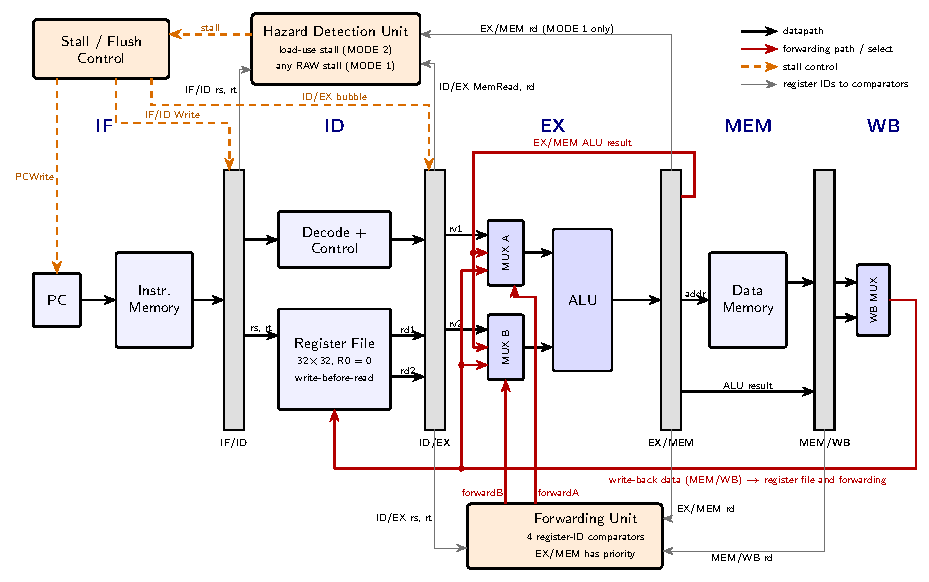
\includegraphics[width=0.95\textwidth]{fig_block_diagram.pdf}
\caption{Block diagram of the five-stage pipeline with the hazard detection unit, stall/flush control, forwarding unit and the two forwarding paths (EX/MEM ALU result and MEM/WB write-back data).}
\label{fig:block}
\end{figure*}

\subsection{Register-ID Comparator}
Every hazard check is built from one comparator:
\begin{equation}
\mathit{match} = W_p \land U_c \land (rd_p \neq 0) \land (rd_p = rs_c),
\end{equation}
where $W_p$ means the producer writes a register, $rd_p$ is its destination, $U_c$ means the consumer really reads this operand, and $rs_c$ is the consumer source register. The $U_c$ term prevents false stalls, for example on the unused \texttt{rt} field of an I-type instruction.

\subsection{Forwarding Unit and Multiplexers}
Four comparators check the EX instruction's \texttt{rs} and \texttt{rt} against the EX/MEM and MEM/WB destinations. The select for each 3:1 operand multiplexer is
\[
\mathit{forward} =
\begin{cases}
10 & \text{EX/MEM match (newest value)},\\
01 & \text{MEM/WB match only},\\
00 & \text{register-file value}.
\end{cases}
\]
EX/MEM has priority because, when both stages write the same register, it holds the newer value (Test~4). For the EX/MEM source, $W_p$ is \textit{RegWrite} $\land\,\lnot$\textit{MemRead}: a load in EX/MEM carries only an address. Operand~B forwarding also supplies SW store data (Test~12).

\subsection{Hazard Detection Unit}
The unit compares the ID instruction against ID/EX and EX/MEM and supports three policies:
\begin{itemize}
\item MODE~0: never stall (incorrect baseline).
\item MODE~1: stall on any RAW dependency with EX or MEM until the producer reaches WB (correct baseline, no forwarding).
\item MODE~2: stall only on a load-use hazard, $\mathit{MemRead}_{ID/EX} \land \mathit{match}(rd_{ID/EX}, rs_{ID}\ \text{or}\ rt_{ID})$.
\end{itemize}

\subsection{Stall/Flush Control}
A stall de-asserts \textit{PCWrite} and \textit{IF/IDWrite}, so the same instruction is fetched and decoded again, and clears all control bits of ID/EX, inserting a bubble. A flush input clears IF/ID and ID/EX; it is tied low in Phase~I and is the hook for branch handling in Phase~II.

\subsection{Verification Strategy}
Table~\ref{tab:verif} summarises the verification. Each system run is checked in three independent ways: (1) a golden model executes the program one instruction at a time and all 31 registers and 256 memory words must match the pipeline; (2) an analytical model of the selected policy predicts the exact number of stall cycles, forwarding events and total cycles; and (3) a monitor checks on every stall that the PC and IF/ID are frozen and a bubble enters ID/EX. To confirm the testbench can find bugs, nine faults were injected into the RTL (e.g. swapped forwarding priority, missing load-use stall, R0 forwarded, missing register-file bypass); all nine were detected. One fault, forwarding a load from EX/MEM, is masked at system level by the load-use stall and was caught only by the forwarding-unit unit test, which shows why both levels are needed.

\begin{table}[t]
\caption{Verification summary (all checks pass)}
\label{tab:verif}
\centering
\begin{tabular}{@{}lr@{}}
\toprule
Test & Checks \\
\midrule
Forwarding unit + comparator + mux & 32{,}192 vectors \\
Hazard detection (3 modes) + stall/flush & 28{,}196 vectors \\
ALU + register file & 40{,}006 + 65 \\
Directed hazard programs, MODE 1 and 2 & 16 + 16 \\
Random 40-instruction programs, MODE 1 and 2 & 100 + 100 \\
MODE 0 directed (expected to fail) & 13 of 16 fail \\
Injected RTL faults detected & 9 of 9 \\
\bottomrule
\end{tabular}
\end{table}

\section{Phase I Progress and Preliminary Results}
The design is written in synthesizable Verilog-2005 \cite{ieee1364}; all RTL modules and testbenches compile with Icarus Verilog \cite{icarus} (\texttt{-Wall}) without warnings. Table~\ref{tab:trace} shows the cycle-by-cycle trace of the load-use case (Test~3) produced by the testbench: the ADD is held in ID for one cycle, a bubble enters EX, and the loaded value is then forwarded from MEM/WB.

\begin{table}[t]
\caption{Pipeline trace of Test 3: LW r1,0(r2); ADD r3,r1,r4 (MODE 2)}
\label{tab:trace}
\centering
\setlength{\tabcolsep}{4pt}
\begin{tabular}{@{}cccccccl@{}}
\toprule
Cycle & IF & ID & EX & MEM & WB & stall & forwarding \\
\midrule
1 & I0 & -- & -- & -- & -- & 0 & \\
2 & I1 & I0 & -- & -- & -- & 0 & \\
3 & I2 & I1 & I0 & -- & -- & 1 & bubble \\
4 & I2 & I1 & -- & I0 & -- & 0 & \\
5 & I3 & -- & I1 & -- & I0 & 0 & A $\leftarrow$ MEM/WB \\
6 & I4 & -- & -- & I1 & -- & 0 & \\
7 & I5 & -- & -- & -- & I1 & 0 & \\
\bottomrule
\end{tabular}
\end{table}

Table~\ref{tab:cpi} compares the stall-only baseline with the proposed design. Cycle counts include the four-cycle pipeline fill; steady-state CPI is $(\text{cycles}-4)/\text{instructions}$. Over all 16 directed tests, execution falls from 214 to 158 cycles (26.2\% fewer, $1.35\times$). On the mixed program (Test~8) stalls drop from 18 to 2 and steady-state CPI from 2.64 to 1.18. On 100 random programs, average CPI falls from 1.462 to 1.136 ($1.29\times$). The remaining stalls are load-use stalls; Test~16 shows that instruction scheduling removes them and reaches the ideal steady-state CPI of 1.00.

\begin{table}[t]
\caption{Performance: stall-only (MODE 1) vs.\ forwarding (MODE 2)}
\label{tab:cpi}
\centering
\setlength{\tabcolsep}{3.5pt}
\begin{tabular}{@{}lrrrrrr@{}}
\toprule
 & \multicolumn{3}{c}{MODE 1} & \multicolumn{3}{c}{MODE 2} \\
\cmidrule(lr){2-4}\cmidrule(l){5-7}
Program (instr.) & cyc & stall & CPI$_{ss}$ & cyc & stall & CPI$_{ss}$ \\
\midrule
T3 LW$\rightarrow$ADD (2) & 8 & 2 & 2.00 & 7 & 1 & 1.50 \\
T8 mixed (11) & 33 & 18 & 2.64 & 17 & 2 & 1.18 \\
T10 LW chain (3) & 11 & 4 & 2.33 & 8 & 1 & 1.33 \\
T15 vec.\ add naive (21) & 43 & 18 & 1.86 & 29 & 4 & 1.19 \\
T16 vec.\ add sched.\ (21) & 34 & 9 & 1.43 & 25 & 0 & 1.00 \\
\midrule
All 16 directed tests & 214 & -- & -- & 158 & -- & -- \\
100 random (avg.\ CPI) & \multicolumn{3}{c}{1.462} & \multicolumn{3}{c}{1.136} \\
\bottomrule
\end{tabular}
\end{table}

\textit{Plan for Phase II.} (1) Add BEQ and control-hazard handling using the flush path; (2) forward a load result from MEM/WB to a dependent store's data input in MEM, removing the stall in Test~9; (3) synthesize the design with Yosys to report area and the timing cost of the forwarding multiplexers; and (4) extend the random tests to longer programs and branches.

\section{Individual Contributions}
\textbf{Jashvitha (team lead):} defined the overall micro-architecture and block diagram; designed the hazard detection unit (MODE 0/1/2), the stall/flush controller and the integrated five-stage pipeline (\texttt{processor\_top.v}); built the system testbench with the golden reference model, analytical timing model, stall monitor and random-program regression; wrote the hazard-detection unit test and the regression script; carried out the CPI comparison; and led the report, video and repository.

\textbf{Chaitanya:} designed the register-ID comparator, the forwarding unit (priority, R0 and load rules) and the operand multiplexers, and wrote the exhaustive forwarding-unit testbench.

\textbf{Palak:} designed the ALU and the register file with write-before-read bypass, wrote their unit testbench, and drafted the literature review.

\textbf{Samarth:} prepared the catalogue of directed hazard test cases and their expected results, created the GTKWave waveform views, and compiled the references.

\bibliographystyle{IEEEtran}
\begin{thebibliography}{99}
\bibitem{patterson2013} D.~A. Patterson and J.~L. Hennessy, \emph{Computer Organization and Design: The Hardware/Software Interface}, 5th~ed. Waltham, MA, USA: Morgan Kaufmann, 2013.
\bibitem{hennessy2017} J.~L. Hennessy and D.~A. Patterson, \emph{Computer Architecture: A Quantitative Approach}, 6th~ed. Cambridge, MA, USA: Morgan Kaufmann, 2017.
\bibitem{kogge1981} P.~M. Kogge, \emph{The Architecture of Pipelined Computers}. New York, NY, USA: McGraw-Hill, 1981.
\bibitem{thornton1964} J.~E. Thornton, ``Parallel operation in the Control Data 6600,'' in \emph{Proc. AFIPS Fall Joint Computer Conf.}, 1964, pp.~33--40.
\bibitem{tomasulo1967} R.~M. Tomasulo, ``An efficient algorithm for exploiting multiple arithmetic units,'' \emph{IBM J. Res. Develop.}, vol.~11, no.~1, pp.~25--33, Jan. 1967.
\bibitem{hennessy1982} J.~Hennessy, N.~Jouppi, S.~Przybylski, C.~Rowen, T.~Gross, F.~Baskett, and J.~Gill, ``MIPS: A microprocessor architecture,'' in \emph{Proc. 15th Annu. Workshop Microprogramming (MICRO-15)}, 1982, pp.~17--22.
\bibitem{hennessy1983} J.~L. Hennessy and T.~Gross, ``Postpass code optimization of pipeline constraints,'' \emph{ACM Trans. Program. Lang. Syst.}, vol.~5, no.~3, pp.~422--448, Jul. 1983.
\bibitem{gibbons1986} P.~B. Gibbons and S.~S. Muchnick, ``Efficient instruction scheduling for a pipelined architecture,'' in \emph{Proc. SIGPLAN Symp. Compiler Construction}, 1986, pp.~11--16.
\bibitem{harris2012} D.~M. Harris and S.~L. Harris, \emph{Digital Design and Computer Architecture}, 2nd~ed. Waltham, MA, USA: Morgan Kaufmann, 2012.
\bibitem{riscv2019} A.~Waterman and K.~Asanovi\'{c}, Eds., \emph{The RISC-V Instruction Set Manual, Volume I: Unprivileged ISA}, RISC-V International, 2019.
\bibitem{hartstein2002} A.~Hartstein and T.~R. Puzak, ``The optimum pipeline depth for a microprocessor,'' in \emph{Proc. 29th Int. Symp. Computer Architecture (ISCA)}, 2002, pp.~7--13.
\bibitem{smith1988} J.~E. Smith and A.~R. Pleszkun, ``Implementing precise interrupts in pipelined processors,'' \emph{IEEE Trans. Comput.}, vol.~37, no.~5, pp.~562--573, May 1988.
\bibitem{ieee1364} \emph{IEEE Standard for Verilog Hardware Description Language}, IEEE Std 1364-2005, 2006.
\bibitem{icarus} S.~Williams, ``Icarus Verilog.'' [Online]. Available: \url{https://steveicarus.github.io/iverilog/}
\end{thebibliography}
\end{document}
